\documentclass[12pt]{article}
\usepackage{tikz}
\usepackage{amsmath}
% Underlining package
\usepackage{ulem}
\usetikzlibrary{angles,quotes}
\usetikzlibrary{intersections}
\usetikzlibrary{arrows.meta}
\usetikzlibrary{calc}
\usepackage[a4paper, portrait, margin=1cm]{geometry}
\usepackage{fancyhdr}

\def \HeadingAnswers {\section*{\Large Name: \underline{\hspace{8cm}} \hfill Date: \underline{\hspace{3cm}}} \vspace{-3mm}
{Parallel lines : Answers} \vspace{1pt}\hrule}

% raise footer with page number; no header
\fancypagestyle{myfancypagestyle}{
  \fancyhf{}% clear all header and footer fields
  \renewcommand{\headrulewidth}{0pt} % no rule under header
  \fancyfoot[C] {\thepage} \setlength{\footskip}{6pt} % raise page number 6pt
}
\pagestyle{myfancypagestyle}  % apply myfancypagestyle

\newcounter{minipagecount}

\begin{document}
\HeadingAnswers
\vspace{8mm}

\begin{minipage}{0.75\textwidth}
  \refstepcounter{minipagecount}
  \noindent{(\theminipagecount)}\quad
  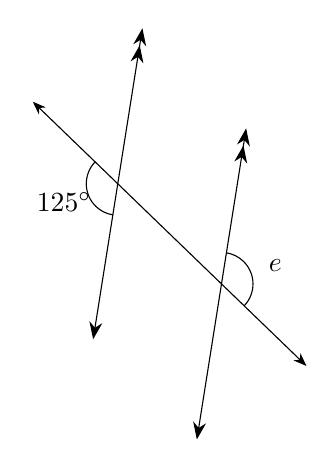
\begin{tikzpicture}[scale=1.0, baseline=(current bounding box.north)]
    \begin{scope}[rotate=316]
      % Draw the first line
      \draw[<->>, >={Stealth[scale=1.3]}, name path=P1] (0, 0) -- (-2.2943057454041846, 3.2766081771559668);
      % Draw the second line with the calculated offsets
      \draw[<->>, >={Stealth[scale=1.3]}, name path=P2] (1.8311618831421843, 0) -- (-0.4631438622620003, 3.2766081771559668);
      % Draw the transversal through the middle of the parallel lines
      \draw[<->, >=Stealth, name path=P3] (-2.647152872702092, 1.6383040885779834) -- (2.184009010440092, 1.6383040885779834);
      
      \path [name intersections={of=P1 and P3,by=A}];
      \path [name intersections={of=P2 and P3,by=B}];

      % Draw the angle
      \coordinate (p1s) at (0, 0);
      \coordinate (p1e) at (-2.2943057454041846, 3.2766081771559668);
      \coordinate (p2s) at (1.8311618831421843, 0);
      \coordinate (p2e) at (-0.4631438622620003, 3.2766081771559668);
      \coordinate (ts) at (-2.647152872702092, 1.6383040885779834);
      \coordinate (te) at (2.184009010440092, 1.6383040885779834);

      % order for vertices go in anticlockwise order te--A--p1e
      \draw pic["$e$", draw=black, -, angle eccentricity=1.8, angle radius=0.4cm] {angle=te--B--p2e};
\draw pic["$125^\circ$", draw=black, -, angle eccentricity=1.8, angle radius=0.4cm] {angle=ts--A--p1s};

      % %% Point A
      % \draw pic["$a$", draw=black, -, angle eccentricity=1.5, angle radius=0.4cm] {angle=te--A--p1e};
      % \draw pic["$b$", draw=black, -, angle eccentricity=1.5, angle radius=0.4cm] {angle=p1e--A--ts};
      % \draw pic["$c$", draw=black, -, angle eccentricity=1.5, angle radius=0.4cm] {angle=ts--A--p1s};
      % \draw pic["$d$", draw=black, -, angle eccentricity=1.5, angle radius=0.4cm] {angle=p1s--A--te};
      
      % %%  Point B
      % \draw pic["$e$", draw=black, -, angle eccentricity=1.5, angle radius=0.4cm] {angle=te--B--p2e};
      % \draw pic["$f$", draw=black, -, angle eccentricity=1.5, angle radius=0.4cm] {angle=p2e--B--ts};
      % \draw pic["$g$", draw=black, -, angle eccentricity=1.5, angle radius=0.4cm] {angle=ts--B--p2s};
      % \draw pic["$h$", draw=black, -, angle eccentricity=1.5, angle radius=0.4cm] {angle=p2s--B--te};

    \end{scope}
  \end{tikzpicture}
\end{minipage}%
\hfill
\begin{minipage}{0.2\textwidth}
  \begin{align*}
    \angle \text{e} &= \text{125}^\circ
  \end{align*}
\end{minipage}
\vspace{1cm}\begin{minipage}{0.75\textwidth}
  \refstepcounter{minipagecount}
  \noindent{(\theminipagecount)}\quad
  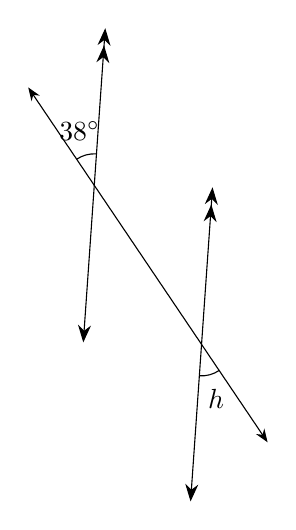
\begin{tikzpicture}[scale=1.0, baseline=(current bounding box.north)]
    \begin{scope}[rotate=304]
      % Draw the first line
      \draw[<->>, >={Stealth[scale=1.3]}, name path=P1] (0, 0) -- (-3.1520430144268876, 2.4626459013026336);
      % Draw the second line with the calculated offsets
      \draw[<->>, >={Stealth[scale=1.3]}, name path=P2] (2.4364038682241156, 0) -- (-0.715639146202772, 2.4626459013026336);
      % Draw the transversal through the middle of the parallel lines
      \draw[<->, >=Stealth, name path=P3] (-3.076021507213444, 1.2313229506513168) -- (2.360382361010672, 1.2313229506513168);
      
      \path [name intersections={of=P1 and P3,by=A}];
      \path [name intersections={of=P2 and P3,by=B}];

      % Draw the angle
      \coordinate (p1s) at (0, 0);
      \coordinate (p1e) at (-3.1520430144268876, 2.4626459013026336);
      \coordinate (p2s) at (2.4364038682241156, 0);
      \coordinate (p2e) at (-0.715639146202772, 2.4626459013026336);
      \coordinate (ts) at (-3.076021507213444, 1.2313229506513168);
      \coordinate (te) at (2.360382361010672, 1.2313229506513168);

      % order for vertices go in anticlockwise order te--A--p1e
      \draw pic["$h$", draw=black, -, angle eccentricity=1.8, angle radius=0.4cm] {angle=p2s--B--te};
\draw pic["$38^\circ$", draw=black, -, angle eccentricity=1.8, angle radius=0.4cm] {angle=p1e--A--ts};

      % %% Point A
      % \draw pic["$a$", draw=black, -, angle eccentricity=1.5, angle radius=0.4cm] {angle=te--A--p1e};
      % \draw pic["$b$", draw=black, -, angle eccentricity=1.5, angle radius=0.4cm] {angle=p1e--A--ts};
      % \draw pic["$c$", draw=black, -, angle eccentricity=1.5, angle radius=0.4cm] {angle=ts--A--p1s};
      % \draw pic["$d$", draw=black, -, angle eccentricity=1.5, angle radius=0.4cm] {angle=p1s--A--te};
      
      % %%  Point B
      % \draw pic["$e$", draw=black, -, angle eccentricity=1.5, angle radius=0.4cm] {angle=te--B--p2e};
      % \draw pic["$f$", draw=black, -, angle eccentricity=1.5, angle radius=0.4cm] {angle=p2e--B--ts};
      % \draw pic["$g$", draw=black, -, angle eccentricity=1.5, angle radius=0.4cm] {angle=ts--B--p2s};
      % \draw pic["$h$", draw=black, -, angle eccentricity=1.5, angle radius=0.4cm] {angle=p2s--B--te};

    \end{scope}
  \end{tikzpicture}
\end{minipage}%
\hfill
\begin{minipage}{0.2\textwidth}
  \begin{align*}
    \angle \text{h} &= \text{38}^\circ
  \end{align*}
\end{minipage}
\vspace{1cm}\begin{minipage}{0.75\textwidth}
  \refstepcounter{minipagecount}
  \noindent{(\theminipagecount)}\quad
  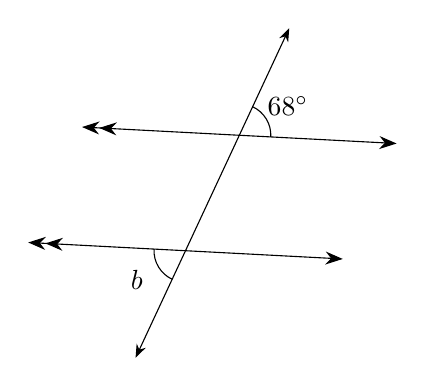
\begin{tikzpicture}[scale=1.0, baseline=(current bounding box.north)]
    \begin{scope}[rotate=65]
      % Draw the first line
      \draw[<->>, >={Stealth[scale=1.3]}, name path=P1] (0, 0) -- (-1.4984263736636483, 3.7087354182671497);
      % Draw the second line with the calculated offsets
      \draw[<->>, >={Stealth[scale=1.3]}, name path=P2] (1.6178021140163752, 0) -- (0.11937574035272691, 3.7087354182671497);
      % Draw the transversal through the middle of the parallel lines
      \draw[<->, >=Stealth, name path=P3] (-2.249213186831824, 1.8543677091335748) -- (2.3685889271845513, 1.8543677091335748);
      
      \path [name intersections={of=P1 and P3,by=A}];
      \path [name intersections={of=P2 and P3,by=B}];

      % Draw the angle
      \coordinate (p1s) at (0, 0);
      \coordinate (p1e) at (-1.4984263736636483, 3.7087354182671497);
      \coordinate (p2s) at (1.6178021140163752, 0);
      \coordinate (p2e) at (0.11937574035272691, 3.7087354182671497);
      \coordinate (ts) at (-2.249213186831824, 1.8543677091335748);
      \coordinate (te) at (2.3685889271845513, 1.8543677091335748);

      % order for vertices go in anticlockwise order te--A--p1e
      \draw pic["$b$", draw=black, -, angle eccentricity=1.8, angle radius=0.4cm] {angle=p1e--A--ts};
\draw pic["$68^\circ$", draw=black, -, angle eccentricity=1.8, angle radius=0.4cm] {angle=p2s--B--te};

      % %% Point A
      % \draw pic["$a$", draw=black, -, angle eccentricity=1.5, angle radius=0.4cm] {angle=te--A--p1e};
      % \draw pic["$b$", draw=black, -, angle eccentricity=1.5, angle radius=0.4cm] {angle=p1e--A--ts};
      % \draw pic["$c$", draw=black, -, angle eccentricity=1.5, angle radius=0.4cm] {angle=ts--A--p1s};
      % \draw pic["$d$", draw=black, -, angle eccentricity=1.5, angle radius=0.4cm] {angle=p1s--A--te};
      
      % %%  Point B
      % \draw pic["$e$", draw=black, -, angle eccentricity=1.5, angle radius=0.4cm] {angle=te--B--p2e};
      % \draw pic["$f$", draw=black, -, angle eccentricity=1.5, angle radius=0.4cm] {angle=p2e--B--ts};
      % \draw pic["$g$", draw=black, -, angle eccentricity=1.5, angle radius=0.4cm] {angle=ts--B--p2s};
      % \draw pic["$h$", draw=black, -, angle eccentricity=1.5, angle radius=0.4cm] {angle=p2s--B--te};

    \end{scope}
  \end{tikzpicture}
\end{minipage}%
\hfill
\begin{minipage}{0.2\textwidth}
  \begin{align*}
    \angle \text{b} &= \text{68}^\circ
  \end{align*}
\end{minipage}
\vspace{1cm}\begin{minipage}{0.75\textwidth}
  \refstepcounter{minipagecount}
  \noindent{(\theminipagecount)}\quad
  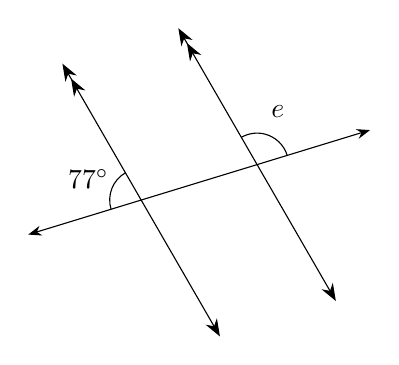
\begin{tikzpicture}[scale=1.0, baseline=(current bounding box.north)]
    \begin{scope}[rotate=17]
      % Draw the first line
      \draw[<->>, >={Stealth[scale=1.3]}, name path=P1] (0, 0) -- (-0.8998042173754601, 3.897480259140941);
      % Draw the second line with the calculated offsets
      \draw[<->>, >={Stealth[scale=1.3]}, name path=P2] (1.5394561616900873, 0) -- (0.6396519443146271, 3.897480259140941);
      % Draw the transversal through the middle of the parallel lines
      \draw[<->, >=Stealth, name path=P3] (-1.9499021086877302, 1.9487401295704705) -- (2.5895540530023573, 1.9487401295704705);
      
      \path [name intersections={of=P1 and P3,by=A}];
      \path [name intersections={of=P2 and P3,by=B}];

      % Draw the angle
      \coordinate (p1s) at (0, 0);
      \coordinate (p1e) at (-0.8998042173754601, 3.897480259140941);
      \coordinate (p2s) at (1.5394561616900873, 0);
      \coordinate (p2e) at (0.6396519443146271, 3.897480259140941);
      \coordinate (ts) at (-1.9499021086877302, 1.9487401295704705);
      \coordinate (te) at (2.5895540530023573, 1.9487401295704705);

      % order for vertices go in anticlockwise order te--A--p1e
      \draw pic["$e$", draw=black, -, angle eccentricity=1.8, angle radius=0.4cm] {angle=te--B--p2e};
\draw pic["$77^\circ$", draw=black, -, angle eccentricity=1.8, angle radius=0.4cm] {angle=p1e--A--ts};

      % %% Point A
      % \draw pic["$a$", draw=black, -, angle eccentricity=1.5, angle radius=0.4cm] {angle=te--A--p1e};
      % \draw pic["$b$", draw=black, -, angle eccentricity=1.5, angle radius=0.4cm] {angle=p1e--A--ts};
      % \draw pic["$c$", draw=black, -, angle eccentricity=1.5, angle radius=0.4cm] {angle=ts--A--p1s};
      % \draw pic["$d$", draw=black, -, angle eccentricity=1.5, angle radius=0.4cm] {angle=p1s--A--te};
      
      % %%  Point B
      % \draw pic["$e$", draw=black, -, angle eccentricity=1.5, angle radius=0.4cm] {angle=te--B--p2e};
      % \draw pic["$f$", draw=black, -, angle eccentricity=1.5, angle radius=0.4cm] {angle=p2e--B--ts};
      % \draw pic["$g$", draw=black, -, angle eccentricity=1.5, angle radius=0.4cm] {angle=ts--B--p2s};
      % \draw pic["$h$", draw=black, -, angle eccentricity=1.5, angle radius=0.4cm] {angle=p2s--B--te};

    \end{scope}
  \end{tikzpicture}
\end{minipage}%
\hfill
\begin{minipage}{0.2\textwidth}
  \begin{align*}
    \angle \text{e} &= \text{103}^\circ
  \end{align*}
\end{minipage}
\vspace{1cm}

\end{document}
